% GNUPLOT: LaTeX picture with Postscript
\begingroup
  \makeatletter
  \providecommand\color[2][]{%
    \GenericError{(gnuplot) \space\space\space\@spaces}{%
      Package color not loaded in conjunction with
      terminal option `colourtext'%
    }{See the gnuplot documentation for explanation.%
    }{Either use 'blacktext' in gnuplot or load the package
      color.sty in LaTeX.}%
    \renewcommand\color[2][]{}%
  }%
  \providecommand\includegraphics[2][]{%
    \GenericError{(gnuplot) \space\space\space\@spaces}{%
      Package graphicx or graphics not loaded%
    }{See the gnuplot documentation for explanation.%
    }{The gnuplot epslatex terminal needs graphicx.sty or graphics.sty.}%
    \renewcommand\includegraphics[2][]{}%
  }%
  \providecommand\rotatebox[2]{#2}%
  \@ifundefined{ifGPcolor}{%
    \newif\ifGPcolor
    \GPcolortrue
  }{}%
  \@ifundefined{ifGPblacktext}{%
    \newif\ifGPblacktext
    \GPblacktextfalse
  }{}%
  % define a \g@addto@macro without @ in the name:
  \let\gplgaddtomacro\g@addto@macro
  % define empty templates for all commands taking text:
  \gdef\gplbacktext{}%
  \gdef\gplfronttext{}%
  \makeatother
  \ifGPblacktext
    % no textcolor at all
    \def\colorrgb#1{}%
    \def\colorgray#1{}%
  \else
    % gray or color?
    \ifGPcolor
      \def\colorrgb#1{\color[rgb]{#1}}%
      \def\colorgray#1{\color[gray]{#1}}%
      \expandafter\def\csname LTw\endcsname{\color{white}}%
      \expandafter\def\csname LTb\endcsname{\color{black}}%
      \expandafter\def\csname LTa\endcsname{\color{black}}%
      \expandafter\def\csname LT0\endcsname{\color[rgb]{1,0,0}}%
      \expandafter\def\csname LT1\endcsname{\color[rgb]{0,1,0}}%
      \expandafter\def\csname LT2\endcsname{\color[rgb]{0,0,1}}%
      \expandafter\def\csname LT3\endcsname{\color[rgb]{1,0,1}}%
      \expandafter\def\csname LT4\endcsname{\color[rgb]{0,1,1}}%
      \expandafter\def\csname LT5\endcsname{\color[rgb]{1,1,0}}%
      \expandafter\def\csname LT6\endcsname{\color[rgb]{0,0,0}}%
      \expandafter\def\csname LT7\endcsname{\color[rgb]{1,0.3,0}}%
      \expandafter\def\csname LT8\endcsname{\color[rgb]{0.5,0.5,0.5}}%
    \else
      % gray
      \def\colorrgb#1{\color{black}}%
      \def\colorgray#1{\color[gray]{#1}}%
      \expandafter\def\csname LTw\endcsname{\color{white}}%
      \expandafter\def\csname LTb\endcsname{\color{black}}%
      \expandafter\def\csname LTa\endcsname{\color{black}}%
      \expandafter\def\csname LT0\endcsname{\color{black}}%
      \expandafter\def\csname LT1\endcsname{\color{black}}%
      \expandafter\def\csname LT2\endcsname{\color{black}}%
      \expandafter\def\csname LT3\endcsname{\color{black}}%
      \expandafter\def\csname LT4\endcsname{\color{black}}%
      \expandafter\def\csname LT5\endcsname{\color{black}}%
      \expandafter\def\csname LT6\endcsname{\color{black}}%
      \expandafter\def\csname LT7\endcsname{\color{black}}%
      \expandafter\def\csname LT8\endcsname{\color{black}}%
    \fi
  \fi
    \setlength{\unitlength}{0.0500bp}%
    \ifx\gptboxheight\undefined%
      \newlength{\gptboxheight}%
      \newlength{\gptboxwidth}%
      \newsavebox{\gptboxtext}%
    \fi%
    \setlength{\fboxrule}{0.5pt}%
    \setlength{\fboxsep}{1pt}%
\begin{picture}(5102.00,4534.00)%
    \gplgaddtomacro\gplbacktext{%
      \csname LTb\endcsname%
      \put(682,704){\makebox(0,0)[r]{\strut{}$-1$}}%
      \put(682,1061){\makebox(0,0)[r]{\strut{}$0$}}%
      \put(682,1417){\makebox(0,0)[r]{\strut{}$1$}}%
      \put(682,1774){\makebox(0,0)[r]{\strut{}$2$}}%
      \put(682,2130){\makebox(0,0)[r]{\strut{}$3$}}%
      \put(682,2487){\makebox(0,0)[r]{\strut{}$4$}}%
      \put(682,2843){\makebox(0,0)[r]{\strut{}$5$}}%
      \put(682,3200){\makebox(0,0)[r]{\strut{}$6$}}%
      \put(682,3556){\makebox(0,0)[r]{\strut{}$7$}}%
      \put(682,3913){\makebox(0,0)[r]{\strut{}$8$}}%
      \put(682,4269){\makebox(0,0)[r]{\strut{}$9$}}%
      \put(814,484){\makebox(0,0){\strut{}$0.5$}}%
      \put(1246,484){\makebox(0,0){\strut{}$1$}}%
      \put(1679,484){\makebox(0,0){\strut{}$1.5$}}%
      \put(2111,484){\makebox(0,0){\strut{}$2$}}%
      \put(2543,484){\makebox(0,0){\strut{}$2.5$}}%
      \put(2976,484){\makebox(0,0){\strut{}$3$}}%
      \put(3408,484){\makebox(0,0){\strut{}$3.5$}}%
      \put(3840,484){\makebox(0,0){\strut{}$4$}}%
      \put(4273,484){\makebox(0,0){\strut{}$4.5$}}%
      \put(4705,484){\makebox(0,0){\strut{}$5$}}%
    }%
    \gplgaddtomacro\gplfronttext{%
      \csname LTb\endcsname%
      \put(176,2486){\rotatebox{-270}{\makebox(0,0){\strut{}$aV(R/a)$}}}%
      \put(2759,154){\makebox(0,0){\strut{}$R/a$}}%
      \put(1703,4096){\makebox(0,0){\strut{}}}%
      \csname LTb\endcsname%
      \put(1606,4096){\makebox(0,0)[r]{\strut{}$\beta=$2.3}}%
      \csname LTb\endcsname%
      \put(1606,3876){\makebox(0,0)[r]{\strut{}$\beta=$3.0}}%
      \csname LTb\endcsname%
      \put(1606,3656){\makebox(0,0)[r]{\strut{}$\beta=$3.5}}%
      \csname LTb\endcsname%
      \put(1606,3436){\makebox(0,0)[r]{\strut{}$\beta=$4.0}}%
      \csname LTb\endcsname%
      \put(1606,3216){\makebox(0,0)[r]{\strut{}$\beta=$4.5}}%
      \csname LTb\endcsname%
      \put(1606,2996){\makebox(0,0)[r]{\strut{}$\beta=$5.5}}%
    }%
    \gplbacktext
    \put(0,0){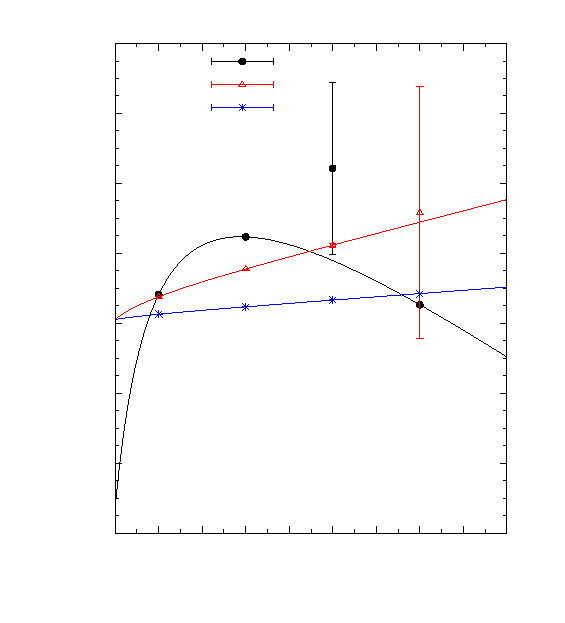
\includegraphics{potentialsu3report}}%
    \gplfronttext
  \end{picture}%
\endgroup
